\chapter{Stereoscopic Video}
\markright{Stereoscopic Video}
\label{stereo_video}
\phantomsection
%\addcontentsline{toc}{chapter}{Stereoscopic Video}









\begin{figure}[h!]
\centering
\begin{subfigure}[]{0.5\textwidth}
		\centering
        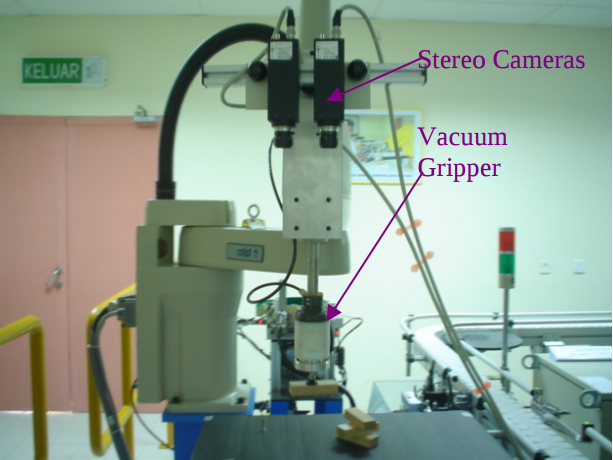
\includegraphics[width=0.7\textwidth]{./img/bin_pick.png}
                \caption{\scriptsize{In bin picking applications stereo vision helps to reconstruct the 3D environment and detect the part of the object to be robotically picked}}
\end{subfigure}% 
~ \quad
\begin{subfigure}[]{0.5\textwidth}
	\centering
	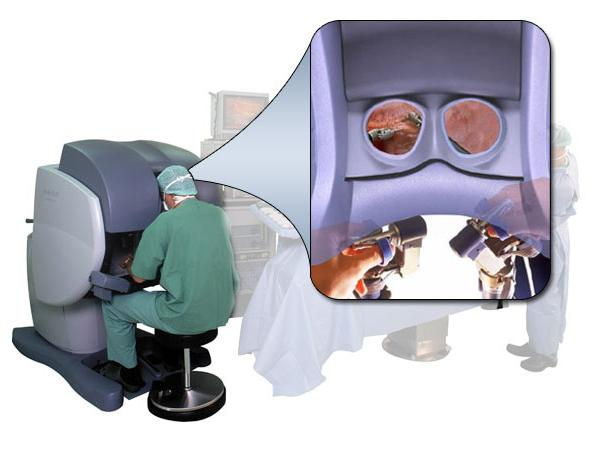
\includegraphics[width=0.7\textwidth]{./img/da_vinci.jpg}
          \caption{\scriptsize{Surgical robot \textit{Da vinci} is provided with a stereoscopic camera that allows a tridimensional view of the operative filed.}}
\end{subfigure} 
\caption{\small{Stereoscopy in medical and industrial field}}
\end{figure}





\begin{figure}[h!]
\centering
\begin{subfigure}[]{0.5\textwidth}
		\centering
        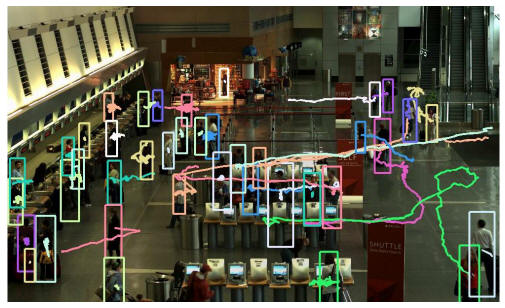
\includegraphics[width=0.7\textwidth]{./img/tracking.jpg}
                \caption{\scriptsize{In people tracking application stereo vision improves segmentation thanks to depth information and it's less sensible to light changes.}}
\end{subfigure}% 
~ \quad
\begin{subfigure}[]{0.5\textwidth}
		\centering
        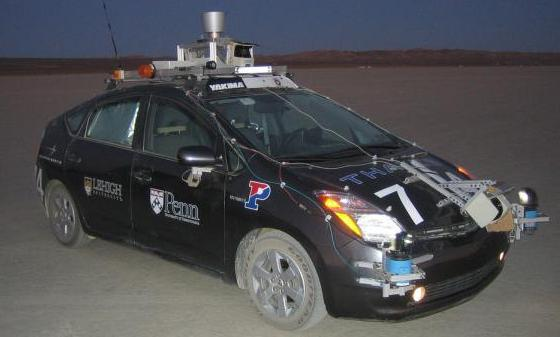
\includegraphics[width=0.7\textwidth]{./img/little_ben.jpg}
                \caption{\scriptsize{In mobile robotics navigation stereo vision has became the first choice technology because it provids a lot of quality data for low costs.}}
\end{subfigure} 
\caption{\small{Stereoscopy application's fields}}
\end{figure}










\begin{figure}[h!]
\centering
\begin{subfigure}[]{0.4\textwidth}
		\centering
        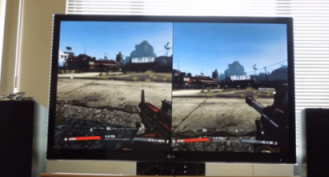
\includegraphics[width=0.7\textwidth]{./img/games1.png}
                \caption{\scriptsize{Stereo video frames, left and right.\newline}}
\end{subfigure}
\begin{subfigure}[]{0.4\textwidth}
		\centering
        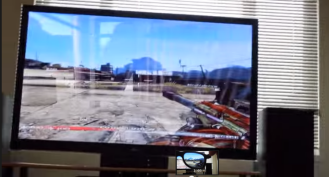
\includegraphics[width=0.7\textwidth]{./img/games2.png}
                \caption{\scriptsize{Overlap of the two frames.}}
\end{subfigure} 
\begin{subfigure}[]{0.4\textwidth}
		\centering
        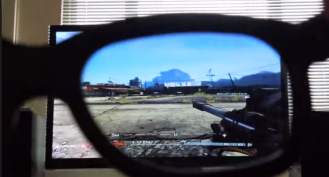
\includegraphics[width=0.7\textwidth]{./img/games3.png}
                \caption{\scriptsize{3D view with specific glasses}}
\end{subfigure}%
\begin{subfigure}[]{0.4\textwidth}
		\centering
        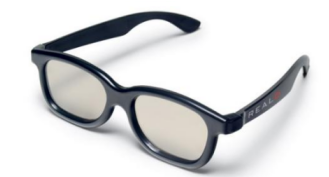
\includegraphics[width=0.7\textwidth]{./img/games4.png}
                \caption{\scriptsize{Polarized glasses for 3D view}}
\end{subfigure} 
\caption{\small{Stereoscopy in 3D video games}}
\end{figure}